\documentclass[letterpaper, 10 pt, conference]{ieeeconf}
\IEEEoverridecommandlockouts
\overrideIEEEmargins
\usepackage{cite}
\usepackage{xcolor}
\usepackage{mathtools}
\usepackage{footnote}
\usepackage{cancel}
\usepackage{xfrac}
\usepackage{amsmath,amssymb,amsfonts}
\usepackage{algorithm}
\usepackage{algorithmicx}
\usepackage{algpseudocode}
\usepackage[hidelinks]{hyperref}
\usepackage{siunitx}
\usepackage{graphicx}
\usepackage{float}
\usepackage{pgf,tikz,pgfplots}
\usepackage{units}
\usepackage{textcomp}
\usepackage[utf8]{inputenc}
\usepackage[english]{babel}

%\pgfplotsset{compat=1.15}
\usepackage{mathrsfs}
\usetikzlibrary{arrows,arrows.meta,automata,calc,intersections,positioning}
\definecolor{sexdts}{rgb}{0.1803921568627451,0.49019607843137253,0.19607843137254902}
\definecolor{dtsfsf}{rgb}{0.8274509803921568,0.1843137254901961,0.1843137254901961}
\definecolor{wrwrwr}{rgb}{0.3803921568627451,0.3803921568627451,0.3803921568627451}
\definecolor{rvwvcq}{rgb}{0.08235294117647059,0.396078431372549,0.7529411764705882}
\definecolor{cqcqcq}{rgb}{0.7529411764705882,0.7529411764705882,0.7529411764705882}

\newtheorem{theorem}{Theorem}
\newtheorem{lemma}{Lemma}

\newcommand{\myparagraph}[1]{\textbf{#1.}}
\renewcommand{\vec}[1]{\ensuremath{\mathbf{#1}}}

\begin{document}

\title{\LARGE \bf
A Minimalistic Approach to Segregation\\
in Robot Swarms}

\author{
  Peter~Mitrano$^{1}$,
  Jordan~Burklund$^{1}$,
  Michael~Giancola$^{1}$,
  Carlo~Pinciroli$^{1}$%
  \thanks{$^{1}$ Robotics Engineering, Worcester Polytechnic Institute, MA, USA. Email: {\sf cpinciroli@wpi.edu}}%
}

\maketitle
\thispagestyle{empty}
\pagestyle{empty}

\begin{abstract}
  We present a decentralized algorithm to achieve segregation into an arbitrary number of groups with swarms of autonomous robots. The distinguishing feature of our approach is in the minimalistic assumptions on which it is based. Specifically, we assume that (i) Each robot is equipped with a ternary sensor capable of detecting the presence of a single nearby robot, and, if that robot is present, whether or not it belongs to the same group as the sensing robot; (ii) The robots move according to a differential drive model; and (iii) The structure of the control system is purely reactive, and it maps directly the sensor readings to the wheel speeds with a simple `if' statement. We present a thorough analysis of the parameter space that enables this behavior to emerge, along with an analysis that explains the emergent behavior. Finally, we study the effect on segregation performance of some non-ideal aspects in the robot morphology.
\end{abstract}

\section{Introduction}

Group formation is one of the most fundamental mechanisms a robot swarm must
exhibit~\cite{Brambilla2013}. Group formation can occur in several forms to
satisfy different requirements. Segregation is a particular type of group
formation in which the focus is on creating local aggregates of robots that
share a common property. Segregation can be seen as a precursor to object
sorting, task allocation, or self-assembly. For example, swarms may need to
split into arbitrary groups to diffuse and search different areas, or segregate
by skill or capability in order to form useful heterogeneous teams.

Segregation is an example of the broader class of spatially organizing
behaviors, whose purpose is to impose a structure in the environment (e.g.,
object clustering~\cite{gauci_clustering_2014}, collective
construction~\cite{Bolger2010}) or in the distribution of the robots (e.g.,
aggregation~\cite{shlyakhov_survey_2017}, pattern
formation~\cite{Pinciroli:DARS2016}, self-assembly~\cite{gross2008self}).

A recent line of research in spatially organizing behaviors focuses on the
\emph{minimal} assumptions a swarm of robots must fulfill in order to perform
the task. Johnson and Brown~\cite{johnson_evolving_2016} and Brown \emph{et
  al.}~\cite{brown_discovery_2018} characterized the set of possible behaviors
that can be obtained using primordial control strategies based on a simple
`if/then/else' structure, binary sensors, and differential-drive robots. Gauci
\emph{et al.} analyzed the emergence of aggregation~\cite{gauci_evolving_2014}
and object clustering~\cite{gauci_clustering_2014}, while St.-Onge \emph{et
  al.}~\cite{StOnge:IROS2018} studied the emergence of circular formations. In
the nascent field of active matter, Lavergne \emph{et al.}~\cite{Lavergne2019}
studied aggregation with active particles equipped with conical sensors capable
of counting the number of detected particles. They analyzed the effect of the
cone angle on the behavior of a swarm of such particles.

While more efficient control strategies have been proposed to achieve these
behaviors, studying the minimal assumptions required for their emergence is an
important step towards principled `swarm engineering' practices. In addition,
these minimal behaviors might offer last-resort solutions in case of sensor
failures in remote environments such as in planetary exploration missions.

This paper furthers this line of inquiry by studying the minimal assumptions for
$N$-class segregation to emerge from local, decentralized interactions among
robots. The term `$N$-class' refers to the creation of $N$ spatially distinct
groups. We show that, for segregation to emerge, it is sufficient to equip an
`if/then/else', differential drive robot with a \emph{ternary} sensor. This
sensor detects the presence of a robot along a line-of-sight. When a robot is detected, the
sensor can distinguish whether it is a \emph{kin}, i.e., it belongs to the same
group as the sensing robot, or a \emph{non-kin}, i.e., it belongs to a different
group. When multiple robots are in range, the sensor returns information on the
closest one of them.

The main contributions of this paper are \emph{(i)} A study of the parameter
space that enables the emergence of $N$-class segregation; \emph{(ii)} A study
of why convergence is guaranteed for the best parameter choice found; and
\emph{(iii)} An analysis of robustness to non-idealities in the robot
morphology.

\section{Related Work}
Segregation is a common behavior in nature, and it can be observed across
scales. For example, cell segregation is a basic building block of embryogeneis
in tissue generation processes~\cite{batlle_molecular_2012,Steinberg1963}; while
social insects, such as ants, organize their brood into ring-like
structures~\cite{Franks1992}.

In robotics, segregation is a problem that has not received considerable
attention. The main methods that have been proposed so far are based on some
variation of the artificial potential approach~\cite{Spears2004}, which assumes
that the robots can detect each other and estimate relative distance vectors.

Gro\ss~\emph{et al.}~\cite{gross_segregation_2009} proposed an
algorithm inspired by the Brazil Nut effect, in which the robots form regular
layers simulating gravity by sharing a common direction. This study was later
extended to work on e-pucks robots~\cite{Chen2012}. To simulate gravity, this
approach requires the robots to share a common target vector, which can be
obtained through centralized controllers or a distributed consensus algorithm.

Kumar \emph{et al.}~\cite{kumar_segregation_2010} introduced the concept of
``differential potential'', whereby two robots experience a different artificial
potential depending on their being part of the same class or not. The
convergence of this approach is guaranteed for two classes, but when more
classes are employed local minima prevent segregation from emerging.

Santos \emph{et al.}~\cite{santos_segregation_2014} took inspiration
from~\cite{kumar_segregation_2010} to devise an approach based on the
Differential Adhesion Hypothesis, which states that kin cells tend to adhere
stronger than non-kin cells. However, one limitation is the assumption
that the robots have global knowledge about the positions of other robots.

To the best of our knowledge, this paper is the first to propose a segregation
algorithm that is not based on global information nor on communication and
sensing of multiple neighbors.

\section{Methodology}

\subsection{Problem Formulation}

\newcommand{\vL}{\ensuremath{v_{\text{left}}}}
\newcommand{\vR}{\ensuremath{v_{\text{right}}}}
\newcommand{\vaL}{\ensuremath{V_{\text{left}}}}
\newcommand{\vaR}{\ensuremath{V_{\text{right}}}}
\newcommand{\VM}{\ensuremath{V_{\text{max}}}}
\myparagraph{Motion model}
We consider a set of robots executing the same controller in a two-dimensional,
obstacle-free environment. The robots are equipped with two wheels for which
$[\vL,\vR]$ denote their \emph{normalized} linear speeds. By `normalized' we
mean that the speed values are in the range $[-1, 1]$. Using normalized speeds
allows us to reason in a general way over the specific speeds attainable by any
robot. To transform from normalized speeds $[\vL,\vR]$ into actual speeds
$[\vaL,\vaR]$, we introduce a parameter $\VM$ that denotes the maximum linear
speed possible with a specific robot and define
\begin{align}
  \vaL &= \VM \vL\\
  \vaR &= \VM \vR.
\end{align}
The robots' motion assuming constant wheel velocities is modeled by the well-known differential-drive
equations, shown in Equation \eqref{eq:motion}.

\newcommand{\vPN}[2]{\ensuremath{v_{\text{#1}}}^{S=#2}}
\newcommand{\robot}[2]{%
  \filldraw[draw=#2,fill=#2!20] (#1) circle(5mm);
  \draw[draw=#2,->,-Stealth,rotate around={0:(#1)}] (#1) -- +(5mm,0);
  \fill[fill=gray!20] ($(#1)+(5mm,0)$) -- +( 45:1cm) -- +(-45:1cm) -- cycle;%
  \fill[fill=#2] ($(#1)+(5mm,0)$) circle (1mm);%
  }

\begin{figure}[t]
  \centering
  \begin{tikzpicture}
    \coordinate (s0) at (0  cm,0cm);
    \coordinate (s1) at (1.5cm,0cm);
    \coordinate (s2) at (3  cm,0cm);
    \robot{s0}{red};
    \robot{s1}{red};
    \robot{s2}{blue};
    \node[below=of s0]{\texttt{S=1}};
    \node[below=of s1]{\texttt{S=2}};
    \node[below=of s2]{\texttt{S=0}};
  \end{tikzpicture}
  \caption{A diagram of the ternary sensor in which classes are depicted
  as colors. The left red robot detects a kin robot, so its sensor
  returns 1. The middle red robot detects a blue robot, so its sensor
  returns 2. The right robot detects no robot, so its sensor returns
  0.}
  \label{fig:sensor}
\end{figure}

\begin{algorithm}[t]
  \begin{algorithmic}
    \If {$S=0$} \State set wheel speeds to $\vPN{left}{0}$, $\vPN{right}{0}$
    \ElsIf {$S=1$} \State set wheel speeds to $\vPN{left}{1}$, $\vPN{right}{1}$
    \Else \State set wheel speeds to $\vPN{left}{2}$, $\vPN{right}{2}$
    \EndIf
  \end{algorithmic}
  \caption{The segregation control algorithm.}
  \label{alg:controller}
\end{algorithm}

\myparagraph{Sensor model}
The robots are also equipped with a ternary sensor that is able to detect the
presence of nearby robots and their ``kinness''. Two robots are \emph{kin} if
they belong to the same class (denoted by color in our experiments); they are
\emph{non-kin} otherwise. The sensor is assumed to have infinite range (we
consider non-infinite range in Sec.~\ref{section:beam_range}). As depicted in
Fig.~\ref{fig:sensor}, the sensor returns a reading $S=0$ when no robot is
detected, $S=1$ when a kin robot is detected, and $S=2$ when a non-kin robot is
detected. We allow for any number of classes, but the sensor need not
distinguish between different non-kin classes---it only detects whether a nearby
robot belongs to the same class or not.

\myparagraph{Control logic}
The control logic followed by the robots is formalized in
Alg.~\ref{alg:controller}. It is a simple `if/then/else' structure, which maps
the sensor readings $S$ directly into normalized wheel speeds $[\,\vL\;\vR\,]$. The
latter are the parameters whose value we intend to study, and they can be
encoded as a six-dimensional vector
$$
[\,
\vPN{left}{0}\;
\vPN{right}{0}\;
\vPN{left}{1}\;
\vPN{right}{1}\;
\vPN{left}{2}\;
\vPN{right}{2}\;
\,].
$$

\myparagraph{Objective}
The objective of our study is to find the values of the speed parameters for
which the robots group into clusters, such that all the robots of the same class
are packed into one cluster with no non-kin robots.

\subsection{Simulation Environment and Robots}

\myparagraph{Simulation platform} We utilized the ARGoS multi-robot
simulator~\cite{pinciroli_argos:_2012} to search for controller parameters and
evaluate them. ARGoS offers accurate models for several differential-drive
robots, such as the foot-bot~\cite{Bonani2010}, the Khepera
IV\footnote{https://www.k-team.com/khepera-iv}, and the
Kilobot~\cite{Rubenstein2012}.

\myparagraph{Simulated Robot platform} For the simulated experiments we opted to
use the foot-bot, because of the possibility to utilize its range-and-bearing
communication system as a base for the ternary sensor. The advantage of using
the range-and-bearing system is that its model is simple and, as a consequence,
a large number of simulations could be completed in a short time. The
range-and-bearing system allows two robots to exchange messages when they are in
direct line-of-sight; upon receiving a message, a robot can also estimate the
relative position of the sender. This sensor, in principle, receives messages
from all the nearby robots. To simulate the ternary sensor, our robot controller
kept the message of the closest robot. The message payload was an integer that
encoded the id of the group to which the sender belonged. The range-and-bearing
sensor is simulated through ray casting. This allowed us to assume that the
sensor reading is infinitely thin, a choice that simplifies the mathematical
analysis presented in Sec.~\ref{sec:analysis}. However, in practical
applications, the sensor can be expected to cast a cone-shaped sensory range
with non-zero aperture angle. We explore the effect of various angles in
Sec.~\ref{sec:aperture_angle}.

\subsection{Grid Search}
\label{sec:gridsearch}

\myparagraph{Trial setup} In order to exhaustively search the space of possible
controllers, we conducted a grid search of the 6-dimensional parameter
space. With respect to a pure optimization approach meant to find the best
parameter setting, grid search has the advantage of characterizing the
segregation performance of the entire parameter space. This, in turn, allows one
to establish how ``easy'' it is to find segregation behaviors, and how they
compare. Due to limited computational resources, we were only able to search
with a resolution of $7$ values per parameter:
$[-1, \sfrac{-2}{3}, \sfrac{-1}{3}, 0, \sfrac{1}{3}, \sfrac{2}{3}, 1]$.  In
total we evaluated $7^6=117,649$ parameter sets. For each parameter set, we
tested 36 different initial configurations (8 with 1-class, 8 with 2-class, 20
with 4-class), with 100 simulated seconds for each trial. These initial
configurations consisted of uniformly random placement, clusters, and lines of
robots distributed throughout the environment. We chose to include some
structured configurations (clusters and lines) because we discovered that they
affected significantly the performance with respect to uniform random
configurations. Hence, by explicitly evaluating diverse initial configurations,
we could better estimate the best parameter values in the general case. Examples
of these starting configurations can be seen in our supplementary
videos.\footnote{\href{https://www.youtube.com/playlist?list=PL9HqYJ1IkIKVX9EsT5BY9LnBsBPTjc5bB}{https://goo.gl/z8UAuB}}

\myparagraph{Clusters}
To define our cost function, we first establish the notion of a cluster.
A cluster can be intuitively defined as an island of connected kin robots,
and we use similar metrics as those use by Gauci \emph{et al.}~\cite{gauci_evolving_2014}.
Denoting with $r$ the radius of the body of a robot, and defining
$\vec{p}_i(t) = [x_i(t)\;y_i(t)]$ as the $x$ and $y$ coordinates of the robot
$i$ at time $t$, we consider any two kin robots to be connected if
\begin{equation} \label{eq:connected}
  \lVert\vec{p}_i(t) - \vec{p}_j(t)\rVert \le 2r + \epsilon \qquad (i \ne j, \epsilon \in \mathbb{R}^+)
\end{equation}
In our experiments, we set $\epsilon = \SI{5}{\centi\meter}$.
We find clusters by first constructing an adjacency matrix and then performing a depth-first search.
Since we are interested in segregating the robots in $N$ classes,
the final result of a trial is expected to be a set of $N$ distinct clusters composed of kin robots.

\myparagraph{Cost function}
To measure the difference between the ideal, perfectly segregated result and any
configuration achieved by the robots over time, we first calculate, for every
class $i$, the number of robots in the largest cluster $K_i(t)$ formed by robots
of class $i$. Since, in principle, different classes might involve different
numbers of robots, in our cost function we employ the ratio
$$
\gamma_i(t) = -\frac{K_i(t)}{k_i}
$$
where $k_i$ is the number of robots that belongs to class $i$. This ratio should
be maximized, so the negative sign assigns larger clusters a lower, more
negative, cost.  At each time step, the cost is
$$
\gamma(t) = \frac{1}{N}\sum_{i=1}^N\gamma_i(t)
$$
Our complete cost function is then
\begin{equation}
  \label{eq:cost_function}
  k_{\text{total}} =  \sum_{t=0}^{T-1} t\gamma(t)
\end{equation}
in which we denote the total trial time with $T$. The effect of multiplying
$\gamma_i(t)$ by $t$ is to highlight the emergence of clusters as the trial time
proceeds: we cannot expect large clusters to be present at the beginning of a
trial, but good parameter settings should grow (and maintain) clusters over
time. In our experiments, we found from visual inspection that
$k_{\text{total}}$ correctly assigns cost in most scenarios.  However, this cost
function considers a straight line of robots to be a cluster, and as such it
might not be ideal for scenarios in which the clusters are required to be tight.

\begin{figure}[t]
  \centering
  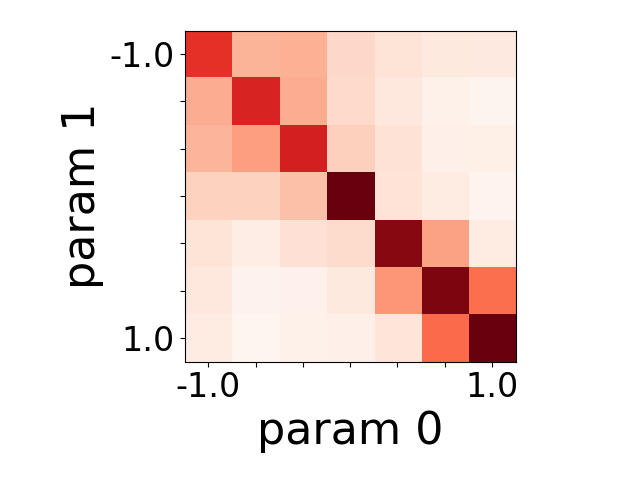
\includegraphics[width=0.24\linewidth]{./images/0_1_grid_img}
  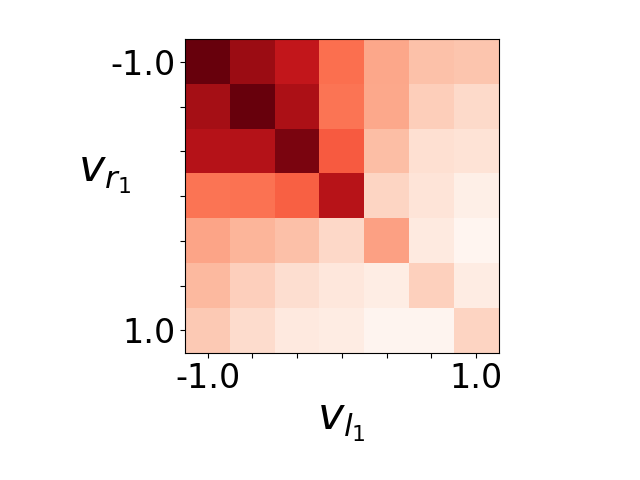
\includegraphics[width=0.24\linewidth]{./images/2_3_grid_img}
  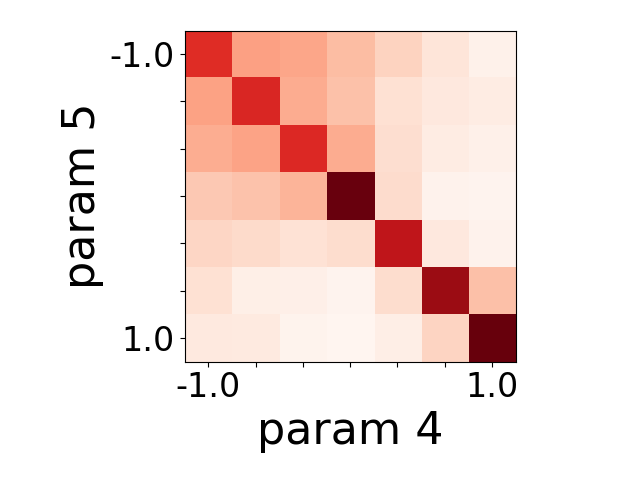
\includegraphics[width=0.24\linewidth]{./images/4_5_grid_img}
  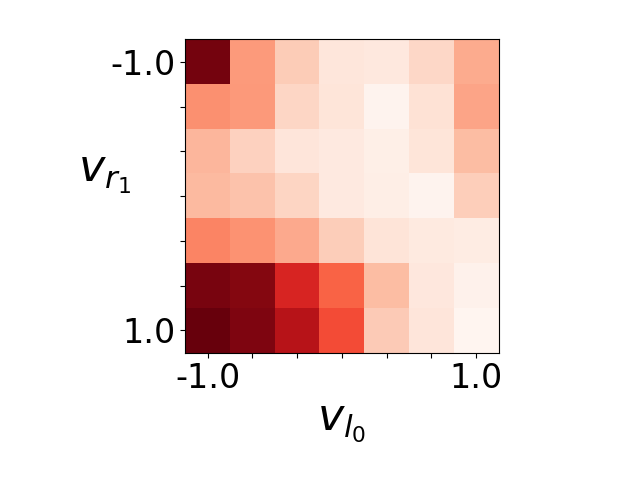
\includegraphics[width=0.24\linewidth]{./images/0_3_grid_img}
  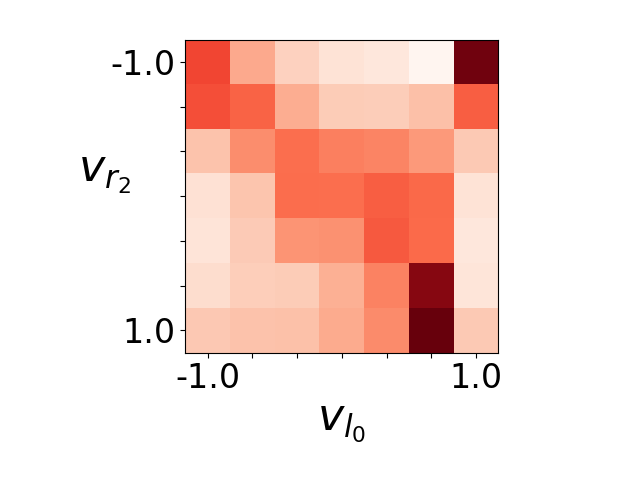
\includegraphics[width=0.24\linewidth]{./images/0_5_grid_img}
  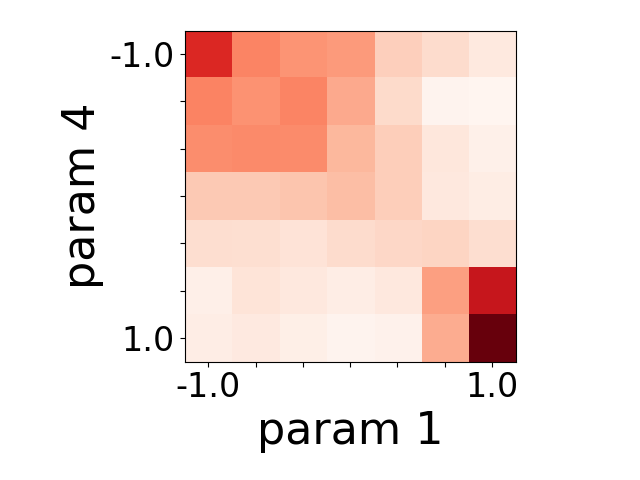
\includegraphics[width=0.24\linewidth]{./images/1_4_grid_img}
  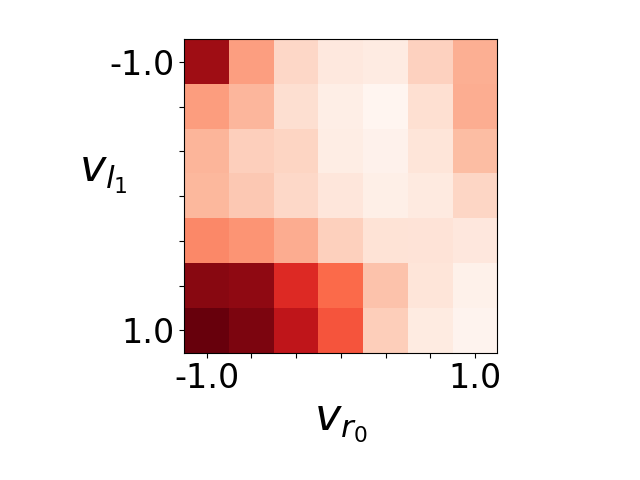
\includegraphics[width=0.24\linewidth]{./images/1_2_grid_img}
  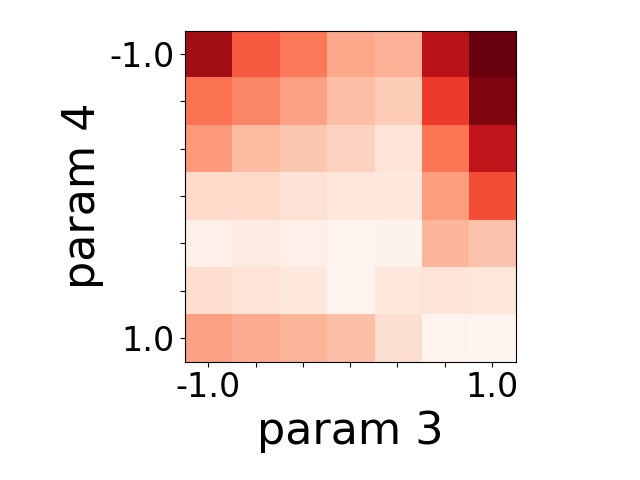
\includegraphics[width=0.24\linewidth]{./images/3_4_grid_img}
  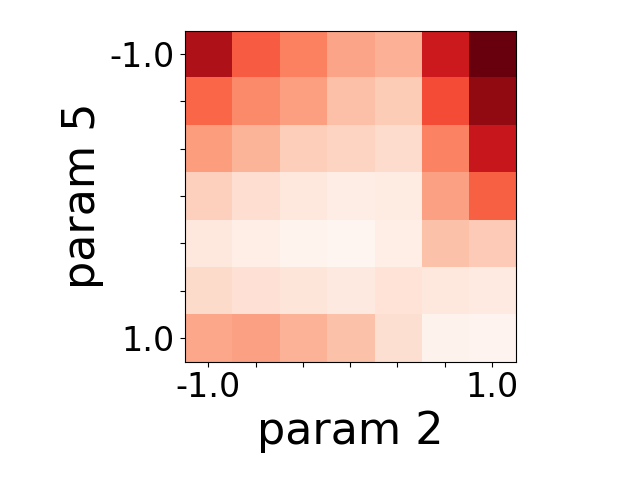
\includegraphics[width=0.24\linewidth]{./images/2_5_grid_img}
  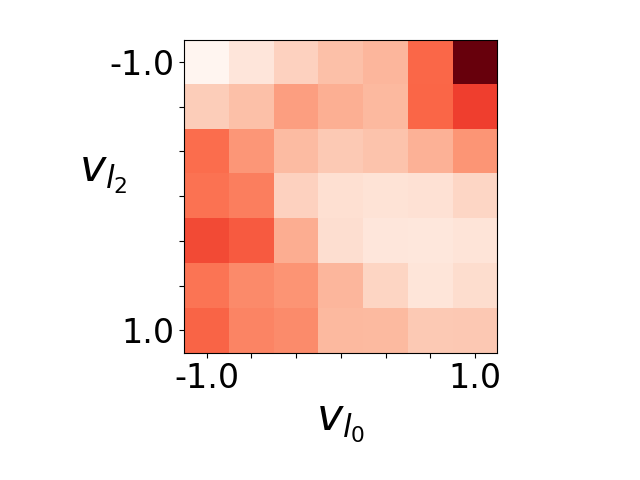
\includegraphics[width=0.24\linewidth]{./images/0_4_grid_img}
  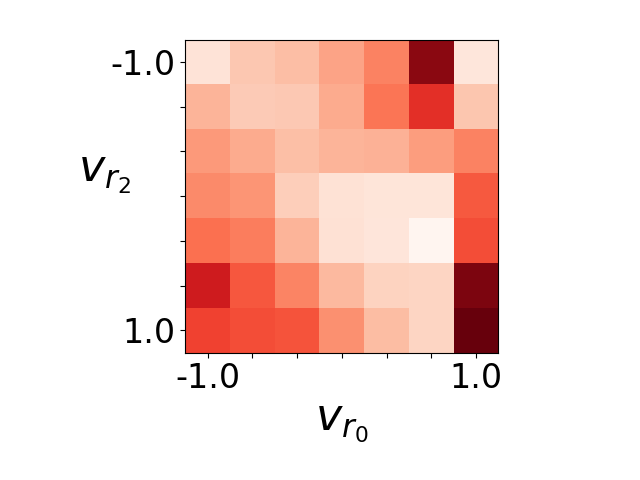
\includegraphics[width=0.24\linewidth]{./images/1_5_grid_img}
  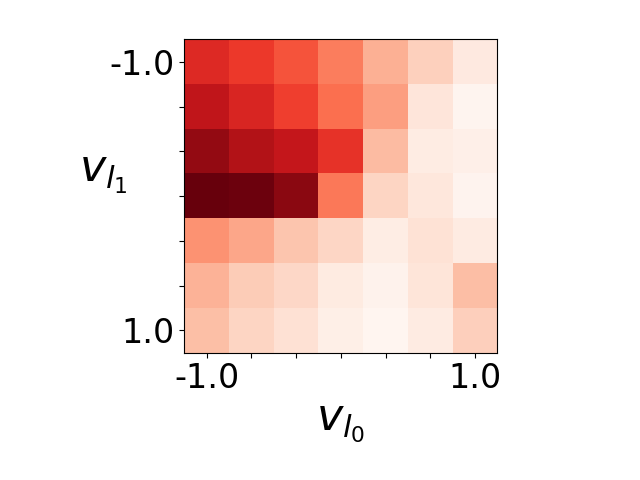
\includegraphics[width=0.24\linewidth]{./images/0_2_grid_img}
  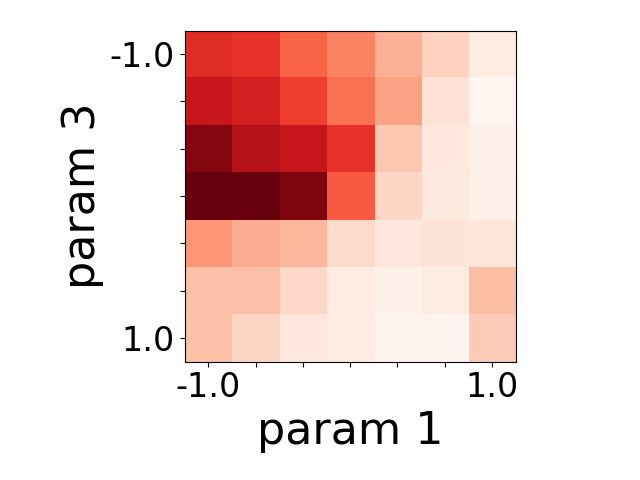
\includegraphics[width=0.24\linewidth]{./images/1_3_grid_img}
  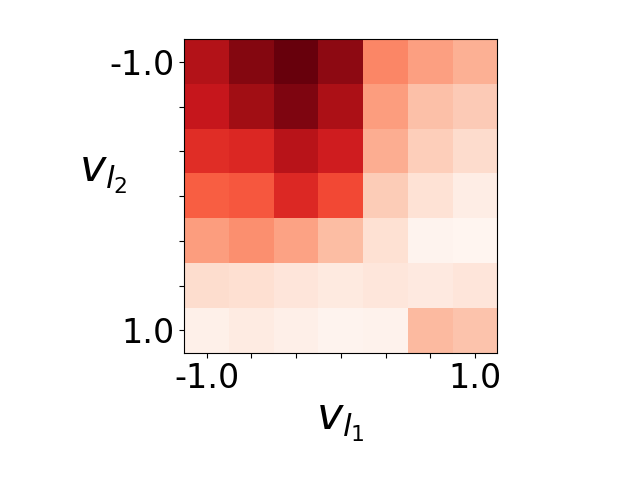
\includegraphics[width=0.24\linewidth]{./images/2_4_grid_img}
  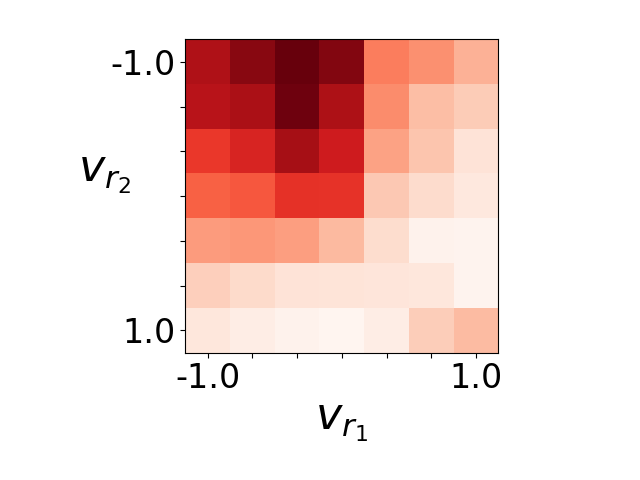
\includegraphics[width=0.24\linewidth]{./images/3_5_grid_img}
  \caption{Heatmaps that relate relevant pairs of wheel speeds. Darker is worse.}
  \label{fig:gridsearch}
\end{figure}

\begin{figure}[b]
  \centering
  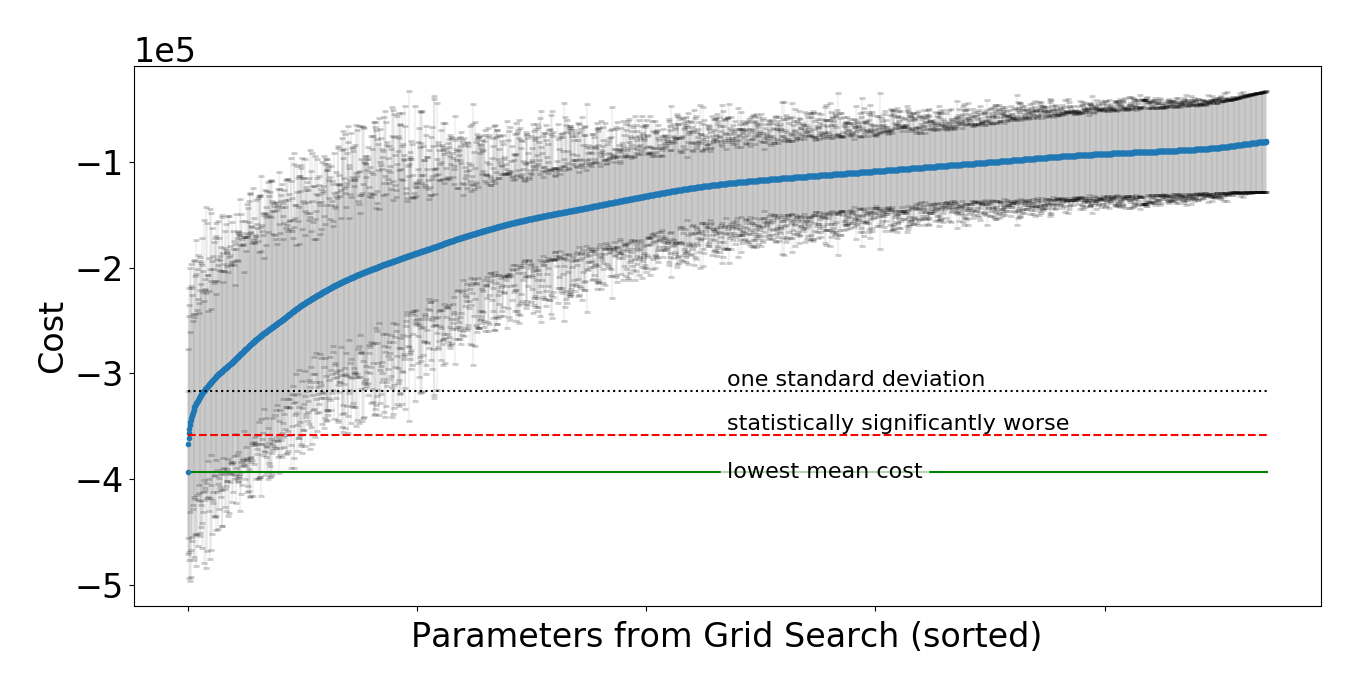
\includegraphics[width=0.9\linewidth]{./images/parameters_distribution.png}
  \caption{The cost of the parameters tested sorted from lowest to (left) highest cost (right).
           The blue line shows the mean cost over all the runs for those parameters, and the graw lines show one standard deviation error bars.
           The black line is the mean of the best paramter setting, the red shows the line above which there is statisticantly significant difference,
           the green line shows one standard deviation, and the darker green line shows two standard devitations.}
  \label{fig:param_dist}
\end{figure}

\section{The Emergent Behavior}
\myparagraph{Visualizing grid search}
The results of grid search are reported in Fig.~\ref{fig:gridsearch}. Because
the search space is six-dimensional, we chose to visualize it by plotting every
pair of parameters against each other. For example, we consider how the cost
changes as $\vPN{left}{0}$ and $\vPN{right}{0}$ change. As an example of reading
these plots, we can tell from the plot of $\vPN{left}{1}$ and $\vPN{right}{1}$
that there were no good controllers where the left and right wheel speeds were
equal and negative (dark squares in the upper left), and that the best
controllers had unequal values close to 1 (lightest squares in the
bottom left). These plots also convey the presence of sharp discontinuities
where performance changes dramatically.

\begin{figure}[t]
  \centering
  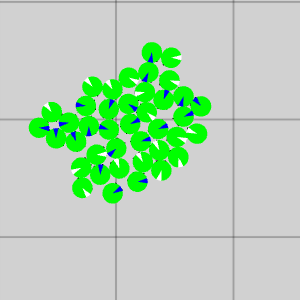
\includegraphics[width=0.32\columnwidth]{./images/segregation_example_1_class_small}
  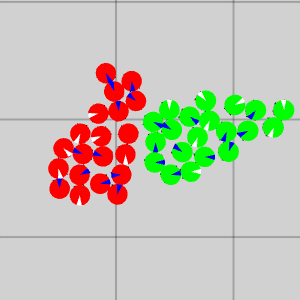
\includegraphics[width=0.32\columnwidth]{./images/segregation_example_2_class_small}
  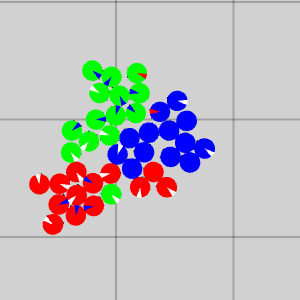
\includegraphics[width=0.32\columnwidth]{./images/segregation_example_3_class_small}\\[1mm]
  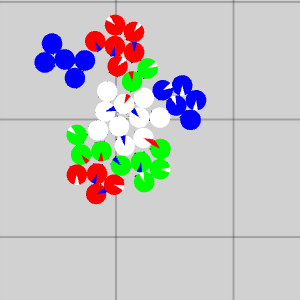
\includegraphics[width=0.32\columnwidth]{./images/segregation_example_4_class_small}
  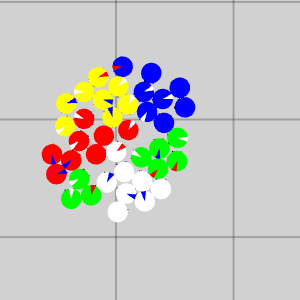
\includegraphics[width=0.32\columnwidth]{./images/segregation_example_5_class_small}
  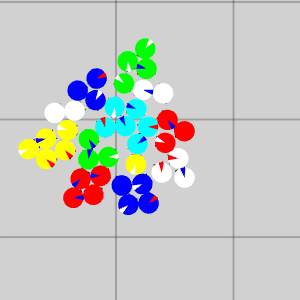
\includegraphics[width=0.32\columnwidth]{./images/segregation_example_6_class_small}
  \caption{Examples of segregation after $\unit[180]{sec}$ with 40 robots
    initially placed at random at a density of 10 robots per square meter.}
  \label{fig:segregation_examples}
\end{figure}

We show the cost of the parameters tested in grid search in Fig.~\ref{fig:param_dist}.
This indicates that most of parameters have statistically significantly higher cost than the best parameters.
However, out of the 117,649 total parameters tested, we found that 126 are not statistically significantly worse.
These include the left-right flipped parameters and as well as controllers which form loops and rings instead of tight clusters.

\myparagraph{The emergent behavior}
After running the grid search, the parameters with the lowest mean cost across all 36
starting configurations were
\begin{equation}
  \label{eq:controller}
  [-1, \sfrac{1}{3}, \sfrac{1}{3}, 1, -1, 1].
  \tag{C}
\end{equation}

The resulting behavior is for a robot to turn sharply until it detects a kin,
then turn less sharply while it sees the kin. This change in the radius of
rotation moves the robot closer to its kin. When a non-kin is seen, the robot
turns in place.  In isolation, the emergent behavior between kin and non-kin is
similar to the aggregation behavior found by Gauci \emph{et
  al.}~\cite{gauci_evolving_2014} in that the robots are always turning in the
same direction (counter-clockwise for our parameters).  In addition, we found
that the best segregation behavior requires that non-kin also aggregate.  This
was not only true for the best parameters, but for all of the top-scoring
parameters we observed.  Examples of the results are shown in Fig.~\ref{fig:segregation_examples}.  To better appreciate the dynamics of this
behavior, we invite the interested reader to watch the videos at
\href{https://www.youtube.com/playlist?list=PL9HqYJ1IkIKVX9EsT5BY9LnBsBPTjc5bB}{https://goo.gl/z8UAuB}.

\section{Behavior Analysis}
\label{sec:analysis}
Using the parameter settings~\eqref{eq:controller}, we now break down and
analyze the emerging behavior, with the aim of explaining why and how
aggregation and segregation occur.

\begin{table}[tb]
  \centering
  \caption{Turning radii and rotational velocities corresponding to the
    parameter settings~\eqref{eq:controller}.}
  \label{tab:omega_and_r}
  \begin{tabular}{c|c|c|c}
             & $S=0$             & $S=1$            & $S=2$           \\
    \hline
    \hline
    $R$       & $\sfrac{-l}{4}$  & $l$              & $0$             \\
    $\omega$  & $\sfrac{4\VM}{3l}$ & $\sfrac{2\VM}{3l}$ & $\sfrac{2\VM}{l}$ \\
    $R\omega$ & $-\sfrac{\VM}{3}$  & $\sfrac{2\VM}{3}$  & $0$             \\
  \end{tabular}
\end{table}

In our analysis, we employ the well-known equations that govern the
instantaneous radius of curvature $R$ and rotation speed $\omega$ of the path
followed a differential-drive robot with $l$ denoting the interwheel
distance~\cite{Dudek2010}:

\begin{equation} \label{eq:motion}
  \begin{aligned}
    R &= \frac{l}{2}\frac{\vaR + \vaL}{\vaR - \vaL} = \frac{l}{2}\frac{\vR + \vL}{\vR - \vL}\\
    \omega &= \frac{\vaR - \vaL}{l} = \frac{\VM(\vR - \vL)}{l}.
  \end{aligned}
\end{equation}

The values of $R$ and $\omega$ corresponding to the
parameters~\eqref{eq:controller} are reported in Table~\ref{tab:omega_and_r}.

\subsection{Robots Aggregate Regardless of Sensor Values}
\label{subsec:analysis_aggregate}
Consider a scenario with two robots $i$ and $j$. For the robot parameters
considered in our experiments, two kin robots in isolation always aggregate
regardless of the value of the sensor readings $S_i$ and $S_j$. Interestingly, two isolated
non-kin robots are also guaranteed to aggregate. We hypothesize that this
aggregation of non-kin is useful for segregation, since by keeping robots close,
kin robots are not initially repelled by non-kin, risking to miss each
other. This is supported by our grid search results, for which we found that the
vast majority of the top-scoring parameters showed aggregation between isolated
non-kin.

\paragraph{$S_i = 0$}
\begin{figure}[t]
  \centering
  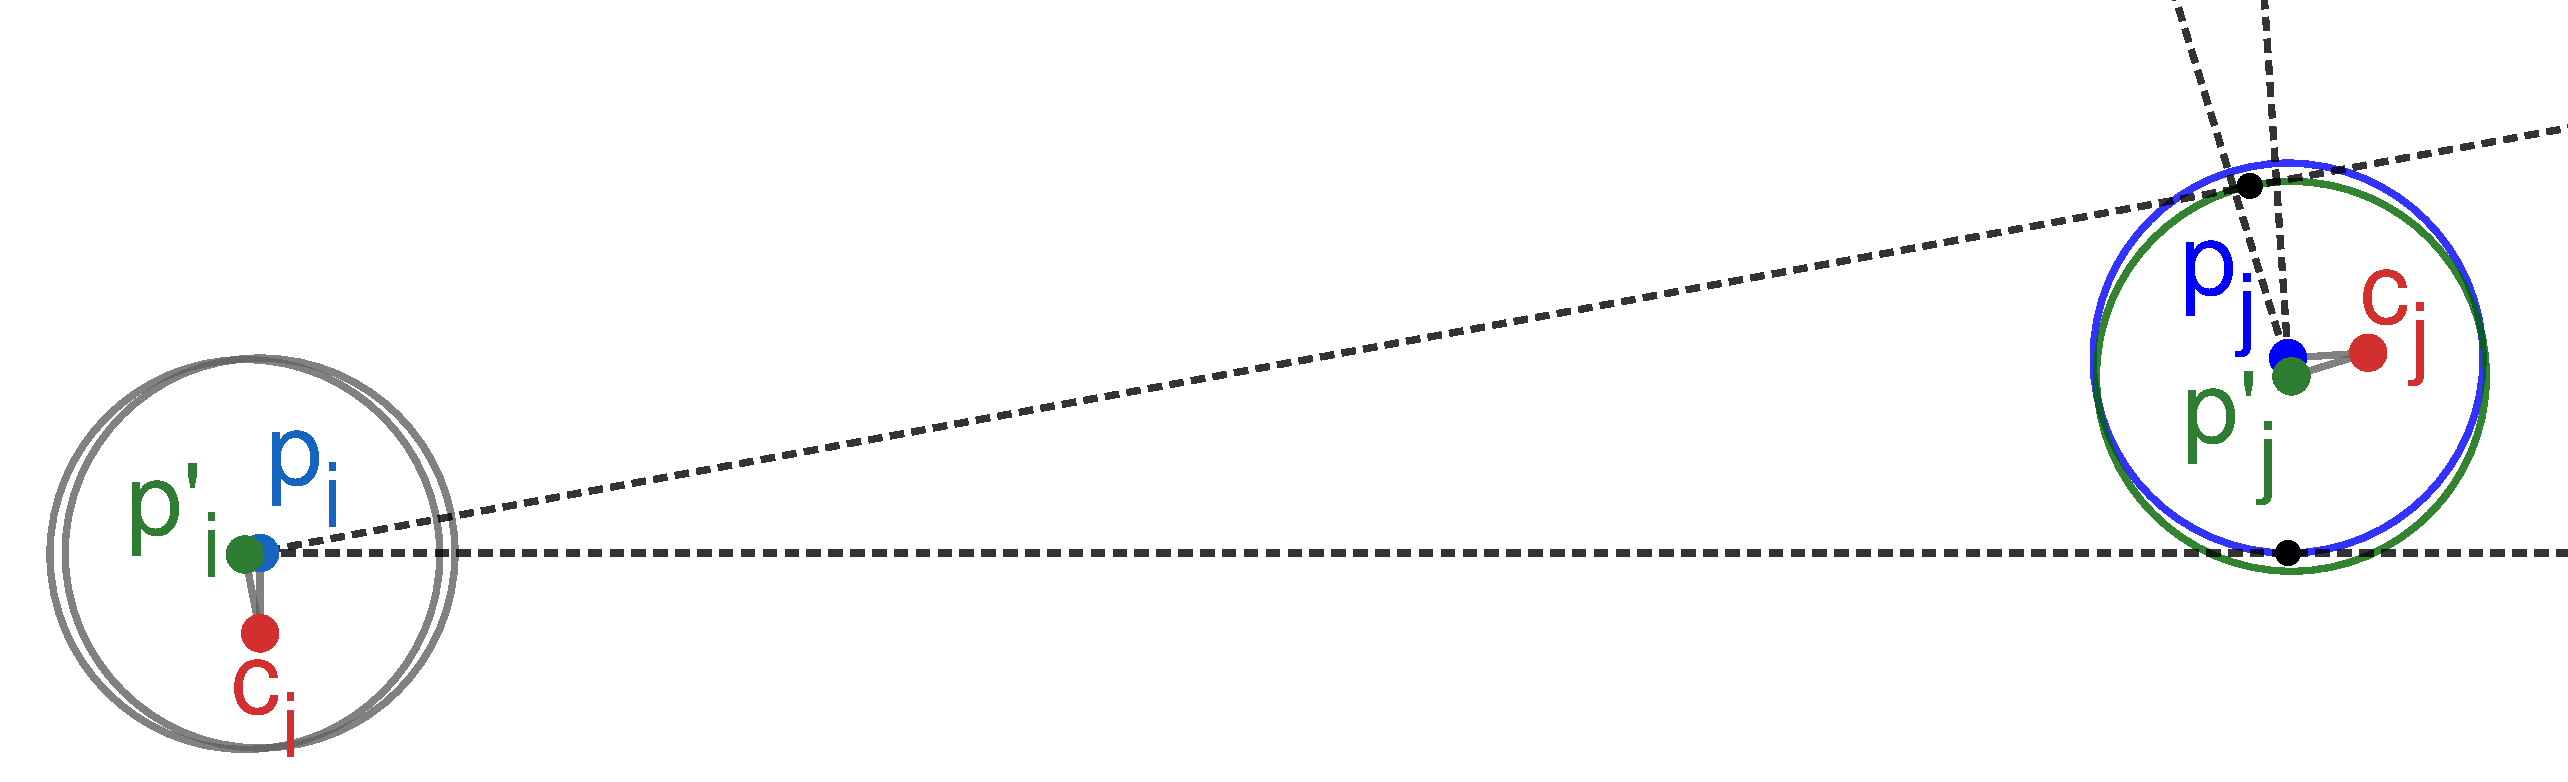
\includegraphics[width=0.8\columnwidth]{./images/thm1}
  \caption{Limit case for $S_i = 0$ and $\Delta t = \unit[100]{ms}$. Robot $i$
    is located at $\vec{p}_i$ and it rotates to $\vec{p}'_i$ around $c_i$. Robot
    $j$ is located at $\vec{p}_j$ and it rotates to $\vec{p}'_j$ around
    $c_j$. The dashed lines indicate the sensor beams of the robots.}
  \label{fig:nothing}
\end{figure}
A sensor value $S_i = 0$ corresponds to the case in which robot $i$ sees
nothing. In the ideal case in which the length of the sensor beam is infinite
and $\Delta t \rightarrow 0$, the beam spans the entire plane. Therefore, the
robot is guaranteed to discover robot $j$. In the non-ideal case in which
$\Delta t$ is not infinitesimally small, the sensor beams are oriented
tangentially and equally distributed along the circular trajectory. For a robot
$j$ to be missed, the arc spanned in $\Delta t$ by $i$'s sensor beam must be
larger than the body of robot $j$, taking into account the fact that $j$
moves. The limit case is reported in Fig.~\ref{fig:nothing} when, at time $t$,
$j$ looks upwards at a certain angle, $S_j = 0$, and $i$'s beam is tangent to
the bottom of $j$'s body. In this case, at $t + \Delta t$ robot $i$'s beam moves
upwards, while $j$'s body moves downwards. For $i$ to miss $j$, the beam at time
$t + \Delta t$ must be tangent to the top of $j$'s body. We used the
\emph{Geometry} package of the GeoGebra
software\footnote{\url{https://www.geogebra.org/}} to numerically solve this
setup, exploiting the fact that we know that both robots rotate by
$\omega^{S=0}\Delta t$. Using the settings in our simulations,
$r = \unit[8.5]{cm}$, $\Delta t = \unit[100]{ms}$, and $\VM = \unit[10]{cm/s}$,
we found the condition $D < \unit[88.8]{cm}$.

\paragraph{$S_i = 1$}
When $i$ sees a kin robot $j$, robot $i$ covers a forwards counter-clockwise
trajectory towards $j$. Along with $i$'s body, also the center of rotation
$C^{S=0}_i$ corresponding to the case $S_i = 0$ moves towards robot $j$. If
$S_j = 0$, its center of rotation $C^{S=0}_j$ stays constant. Therefore, if
robot $i$ experiences $S_i = 0$ at $t + \Delta t$, its rotation around
$C^{S=0}_i$ will be closer to $C^{S=0}_j$. Repeating this over time, the two
robots will aggregate. If instead $S_j = 1$, because we are considering the case
of two isolated robots, the robots move towards each other, again eventually
forming an aggregate.

\paragraph{$S_i = 2$}
When $i$ sees a non-kin robot $j$, robot $i$ rotates counter-clockwise on the
spot. Analogously to $S_i = 1$ case, the center of rotation $C^{S=0}_i$ moves
towards robot $j$ due to this rotation, although much less than in the previous
case. This fosters an aggregation process that is identical in style to the
$S_i = 1$ case, but proceeding at a much slower rate.

\subsection{Robot Segregation}
\label{subsec:analysis_aggregate}

Proving analytically why segregation occurs is difficult. In this section, we
provide a qualitative explanation, leaving a formal proof to future research.

First, consider the motion of an already formed aggregate of robots. Because of
the counter-clockwise rotation that every robot experiences regardless of the
sensor reading, an aggregate also rotates counter-clockwise.

However, because of the different radii of rotation due to the different values
of the sensor readings, the robots do not rotate in the same way. In particular,
when $S=0$ and $S=1$, the robots rotate in opposite directions (respectively
backwards counter-clockwise and forwards counter-clockwise), while when $S=2$
the robots turn on the spot. These differences promote mixing among the robots.

In addition, a robot with $S=1$ moves towards the kin robot detected. Therefore,
when an aggregate comes in contact with another kin aggregate due to mixing, the
two aggregates tend to merge. In contrast, a robot with $S=2$ rotates on the
spot, thus staying with the current aggregate rather than moving away from
it. As a consequence, kin aggregate merging is more effective than non-kin
aggregate merging, i.e., aggregate disruption. The latter occurs occasionally
only due to the random fluctuations caused by the mixing motion of the
aggregate. Thus, in the long run, kin aggregates are likely to form and maintain
their stability.

\section{Experimental Results}

\subsection{Scalability Study} \label{section:scalability}

We investigated how the segregation behavior scales with the number of classes
and the number of robots in the environment. We varied the number of classes
from 1 to 25 and ran 100 trials with robots uniformly randomly distributed. All
trials lasted 180 seconds.

\myparagraph{Fixed number of robots per class}
We studied the case in which every class has 10 robots. The results of this are
plotted in Fig.~\ref{fig:num_classes_10}. We observe that the cost increases
with the number of classes. As the number of classes increases,
the density of the robots increases too. Hence, line-of-sight occlusions between robots are more likely,
navigation is more difficult, and the clusters do not have a chance to coalesce.
The important trend is that as the number of robots increases, the cost increase sublinearly.
This suggests that our method scales well with the total number of robots.

\myparagraph{Fixed total number of robots}
We considered the scenario in which a fixed number of robots is split into an
increasing number of classes. We set the number of robots to 100, so with 25
classes 4 robots were still assigned to each class. As reported in
Fig.~\ref{fig:num_classes_100}, the cost is very low for small numbers of classes
and above 5 classes has no trend in cost. The initial low cost is due to the fact that
with 100 robots to divide among few classes, line-of-sight to a kin is highly likely.
This trend indicates that our algorithm scales well with the number of classes.

\begin{figure}[t]
  \centering
  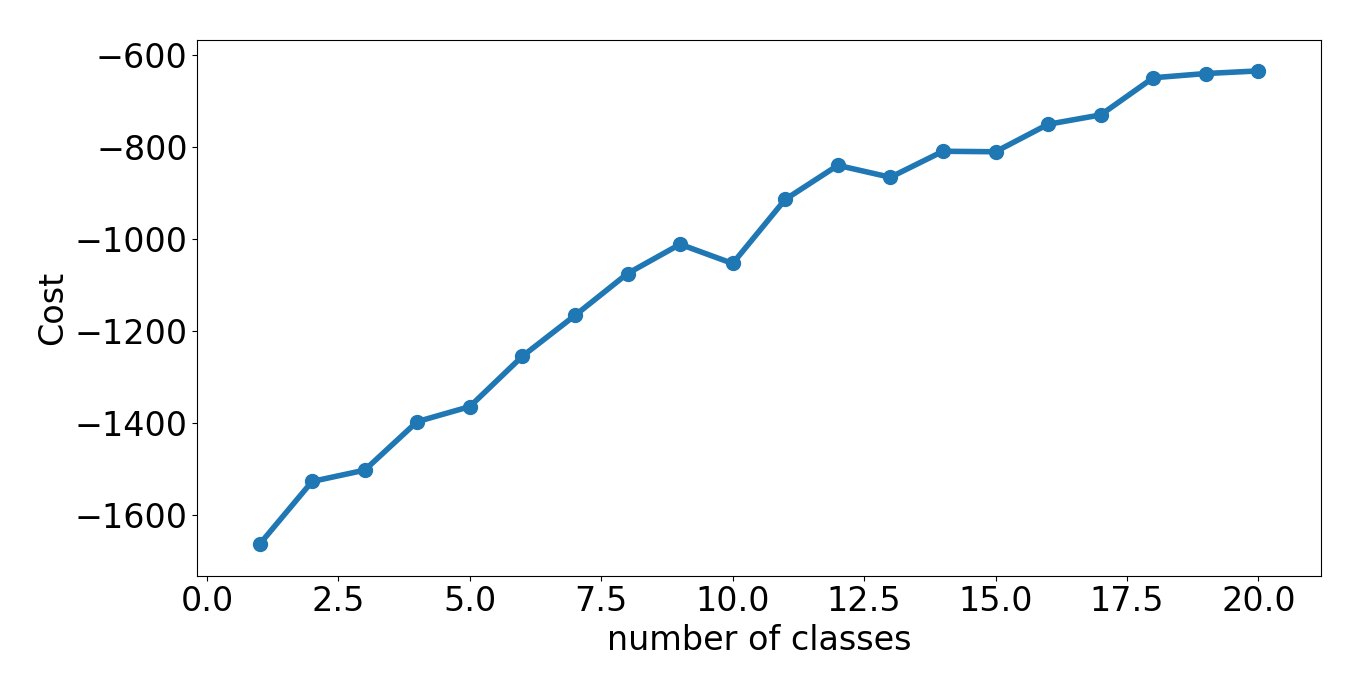
\includegraphics[width=0.9\linewidth]{./images/num_classes_vs_cost_10_per_class}
  \caption{The cost over 100 trials with $N$ classes, 10 robots per class. The
    boxplots indicate the minimum, maximum, interquartile range and median of
    the data distribution. The continuous line connects the medians.}
  \label{fig:num_classes_10}
\end{figure}

\begin{figure}[t]
  \centering
  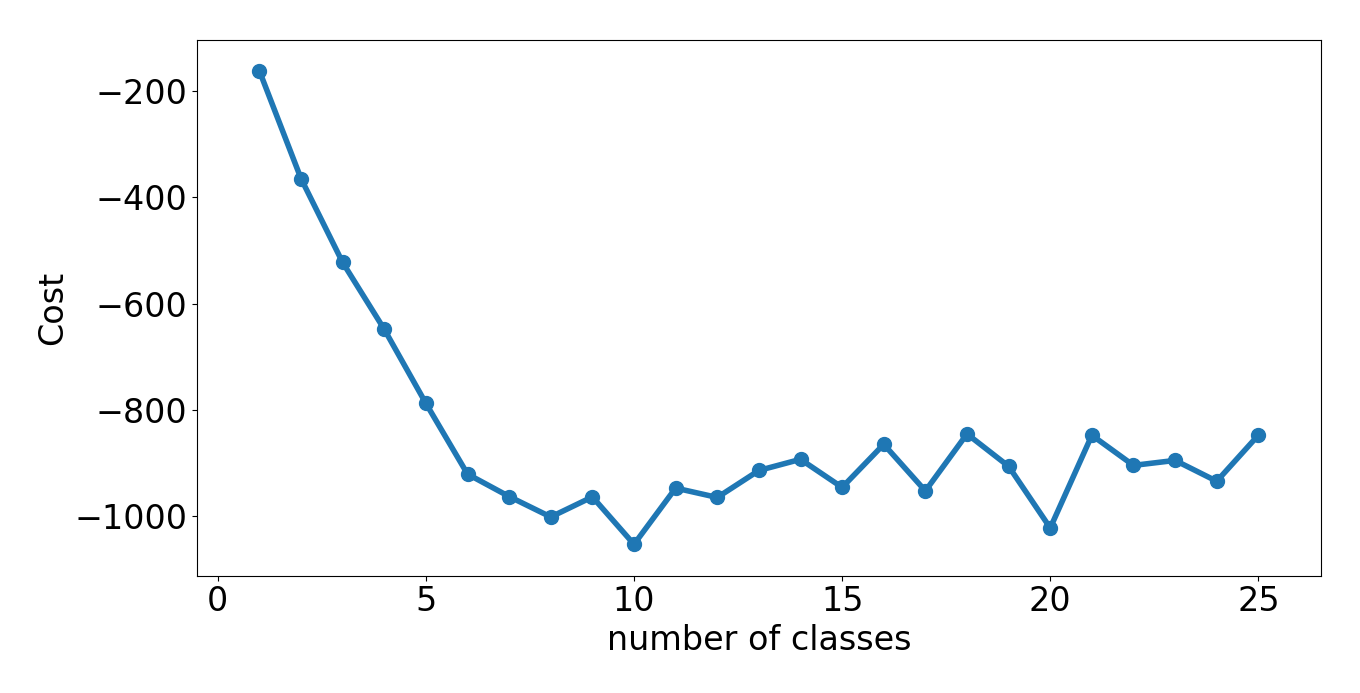
\includegraphics[width=0.9\linewidth]{./images/num_classes_vs_cost_100_robots}
  \caption{The cost over 100 trials with 100 robots divided into $N$
    classes. The boxplots indicate the minimum, maximum, interquartile range and
    median of the data distribution. The continuous line connects the medians.}
  \label{fig:num_classes_100}
\end{figure}

\subsection{The Effect of Implementation Details of the Sensor} \label{section:sensor_impl}

We observed that the implementation details of the sensor have a significant
effect on the robot behavior.

Initially, our method for determining sensor value from the simulated
range-and-bearing system was to consider all the robots within some small angle
in front of the robot and pick the closest one. This is very similar to what
would be provided by a real-world camera that uses colored skirts on each robot
and picks the largest blob as the robot to be detected. This sensor
implementation works well and was used in all our experiments. However, we found
later that, if the robots instead always prefer to react to kin over non-kin,
clusters form more quickly and robustly. For example, if there are two robots
within the field of view of a robot's sensor and the non-kin robot is closer,
the robot would ignore it and execute the $S=1$ logic, which drives the robot
towards the farther kin robot. Exploring exactly which of the various
implementation details have what effect on cost is left for future work.

\subsection{The Effect of the Beam Angle} \label{sec:aperture_angle}

On a real robot, there must be some finite beam angle to the theoretically
line-of-sight sensor. We ran 100 trials with a duration of 180 simulated seconds
with uniformly random initial distributions of 40 robots and various beam
angles. The results are reported in Fig.~\ref{fig:beam_angle}, along with a
diagram showing how we define beam angle. The best beam angle we tested was
\ang{20}, and angles smaller or larger became progressively worse. We found that
at lower beam angles, the robots would segregate very slowly. This is because a narrow beam
means kin are only sensed for one or two consecutive steps.
For larger beam angles, once a robot finds a kin is can almost always reads $S=1$
and gets ``stuck'' with the kin instead of peeking around them to find other kin.

\begin{figure}[t]
  \centering
  \begin{tikzpicture}[scale=0.75]
    \draw (0,0) circle (0.75);
    \draw (0,0) -- (5,0.7);
    \draw[dashed] (0,0) -- (5,0);
    \draw (0,0) -- (5,-0.7);
    \draw (4,0) arc [radius=4, start angle=0, end angle=8];
    \node at (4.25,0.25) {$\beta$};
  \end{tikzpicture}
  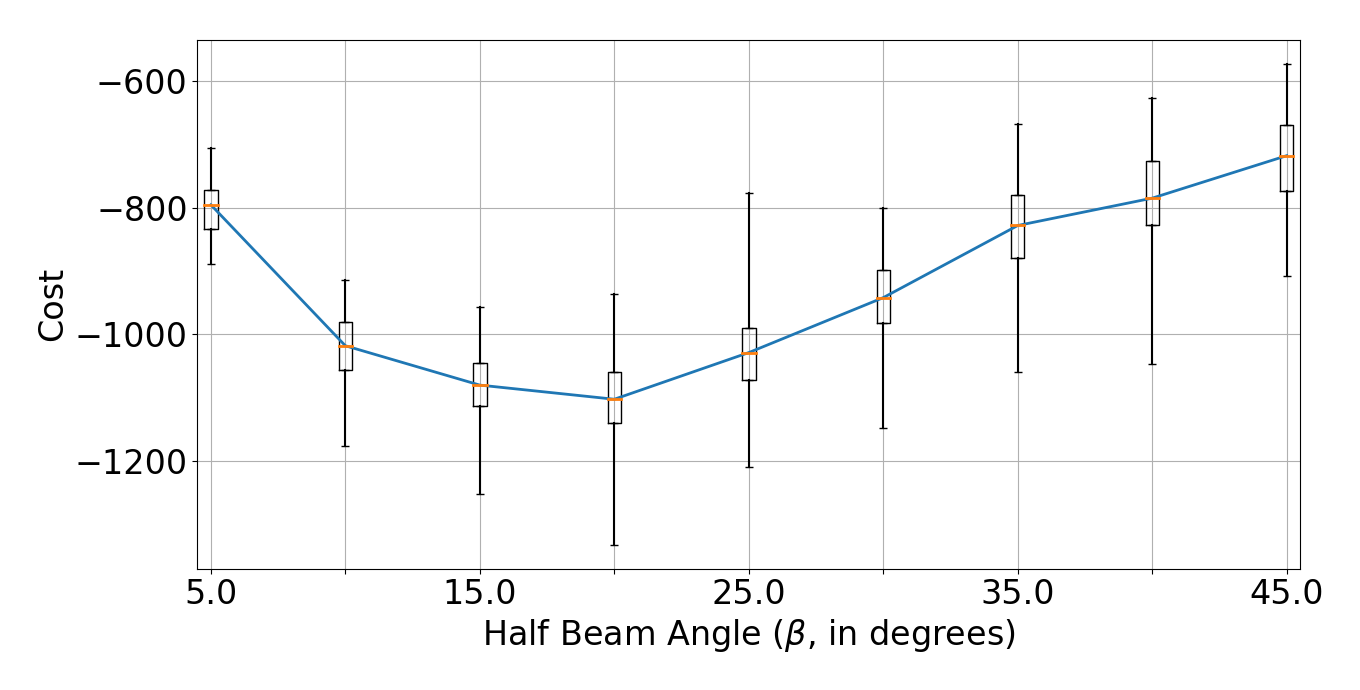
\includegraphics[width=0.9\linewidth]{./images/beam_angle}
  \caption{A \ang{20} degree half beam angle is best for segregation. Lower cost
    is better.}
  \label{fig:beam_angle}
\end{figure}

\subsection{The Effect of Beam Length} \label{section:beam_range}

We consider what happens if the theoretically infinite-range sensor has finite
range. We use \ang{15} half beam angle and the same experimental setup as with
the beam angle experiments. We consider the maximum range of the sensor as the
diagonal length of the square in which the robot are initially distributed. In
all our experiments, this square was \SI{5}{\meter} on each side, so we consider
a range of \SI{7.07}{\meter} to be effectively unlimited. We report the costs
for beam ranges as a fraction of this maximum range. As shown in
Fig.~\ref{fig:beam_range}, a beam range of 25\% of the theoretical maximum
performs just as well as an infinite sensor. Below this, the performance
degrades.

\begin{figure}[t]
  \centering
  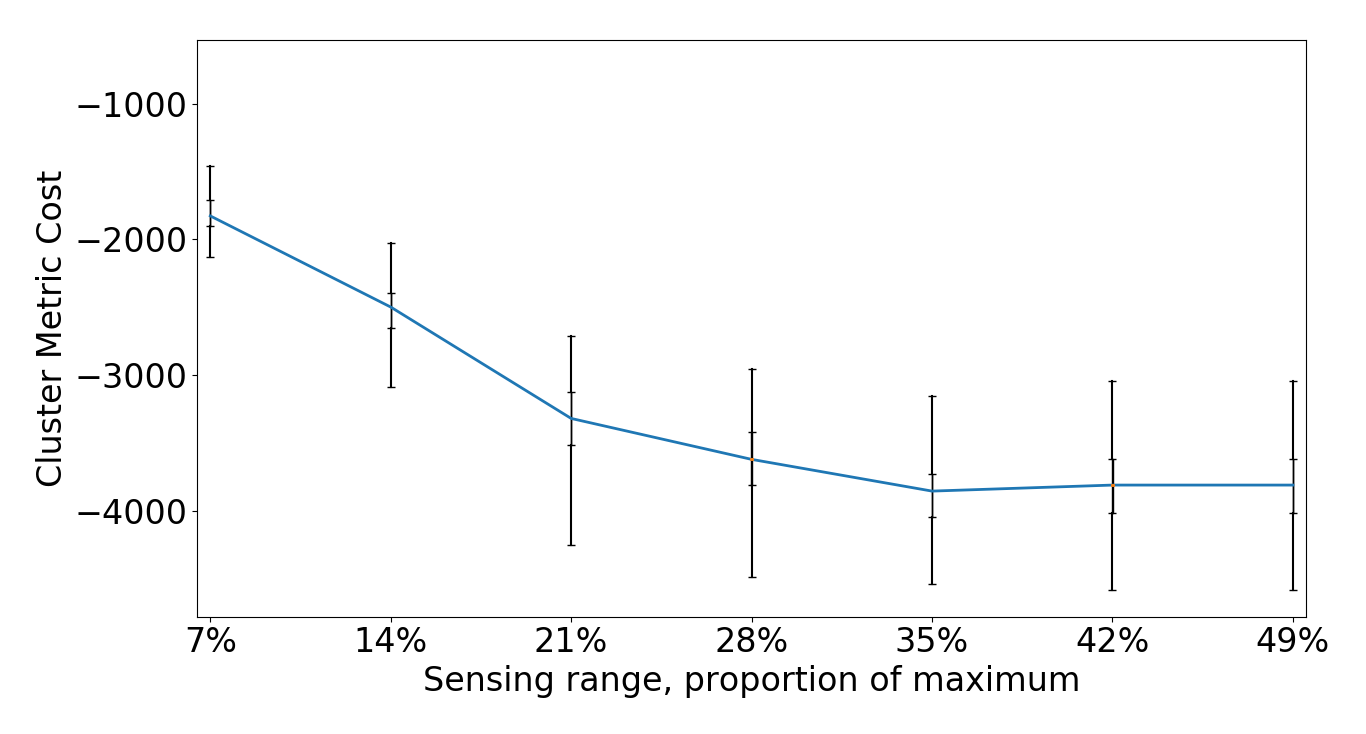
\includegraphics[width=0.9\linewidth]{./images/beam_length}
  \caption{Segregation is robust to small sensor beam ranges. The performance at
    25\% of maximum range is indistinguishable from infinite range.}
  \label{fig:beam_range}
\end{figure}

\section{Conclusion}

In this paper, we show how robots with a simple ternary sensor capable of
detecting kinness and a controller which maps sensor readings to wheel speeds
reactively is capable of $N$-class segregation. We performed a grid search to
characterize the parameter space, and we investigated the effect of sensor
implementation details and the number of robots and classes on performance. Our
findings indicate that, despite the simplicity of our approach, $N$-class
segregation emerges and is fairly robust to these non-idealities in the
morphology of the robot. In addition, we observed that our approach scales well
with the number of robots and the number of classes considered. Building upon
these results, future work will investigate the coordinated behaviors that
emerge when the robots are allowed to change their class dynamically.

\bibliographystyle{IEEEtran}
\bibliography{RBE595.bib}

\end{document}
